\chapter{Part II: Storage Format Enhancement}
\label{chap:storage-format}
In the previous chapter, we concluded that there was potential in column storage in \gap, but that more memory could be saved by enhancing the data storage format. In this chapter, we show how memory usage is reduced and memory locality improved by replacing \cn{GValue}s with primitive data types. We also study the effect of loading raw string values from XML directly into the columns.

This chapter forms the second iteration of our design and experiment part of the research. In this iteration, we are mainly pursuing reduced memory footprint, but the modifications from the storage format enhancements serve as an important foundation for column operations, which we discuss in Chapter \ref{chap:operations}.  
\clearpage

\section{Introduction}
\label{sec:Introduction}
In Section \ref{sec:Challenges in Genus App Platform}, we saw that two of the challenges in the original \gap~data representation are poor memory locality and inefficient storage usage. Both challenges are caused by the \cn{GValue} class. In this structure, data is stored inefficiently due to overhead of pointers and reference counting. For example, it takes 24 bytes to store a 4 byte integer. Secondly, since \cn{GValue} is a class type, it is heap allocated by the memory manager, and we have no control over where the values reside in memory. In Chapter \ref{chap:olap}, we saw that spatial and temporal locality is paramount for performance.

One might think that cache locality has been improved by the introduction of \cn{FieldValueCollection} in the previous chapter. This is only partially true; we store value pointers consecutively in memory with the \cn{TArray} type, but the structures containing the data itself reside in arbitrary memory locations.

Section \ref{sub:Delphi Types} explained that \delphi~supports a wide range of simple, or primitive, data types. These include integer, character, Boolean, real, and more. Common for these data types is that they are value types and a variable with one such type stores the data directly, and not as a pointer. This is also the case for the \delphi~\cn{record} type.

Our observation is simple. If we change the value buffers in \cn{FieldValueCollection} from holding \cn{GValue} references to storing primitive value types directly, we overcome the above challenges. First, we reduce memory consumption by transitioning to primitive data types, since these values have no pointer or reference counting overhead associated with them. Second, since we plan to store the values directly in \delphi~array structures, we improve memory locality.

The data source loading mechanism in \gap~operates using \cn{GValue}s, but since this class is no longer used to store data, we are curious to see whether \cn{GValue}s can be eliminated from the data load process. We believe data load time can be reduced by loading the database values directly from XML instead of using \cn{GValue}s as temporary storage.


Motivated by the memory reduction and the ability to regain control over memory, we create a new structure based on the \cn{FieldValueCollection} interface, which we denote as \cn{PrimitiveFieldValueCollection}. We also circumvent \cn{GValue} creation in the \gap~load module and pass raw XML values directly to the columns. We hypothesize that these changes will reduce memory consumption and increase load time.
\section{Implementation}
\label{sec:Implementation}
In this section, we start by explaining the \cn{PrimitiveFieldValueCollection} class, and how \gap~selects the correct column type. Then we elaborate on how we circumvent the creation of \cn{GValue}s in the data load module.

\subsection{PrimitiveFieldValueCollection}
\label{sub:PrimitiveFieldValueCollection}
We propose not to store \cn{GValue} instances within the columns, but rather as primitive data types. However, since the column operations still use \cn{GValue} in its access methods, the data has to be extracted from these instances on its way in, and new \cn{GValues} must be created on the way out. In this research, we refer to these simple data types as \textit{Primitive Data Types}. 

\afigure{img/primitive-hierarchy.png}{Column store hierarchy after the introduction of primitive data types. \cn{FieldValueCollection} and \cn{PrimitiveFieldValueCollection} extends a base class. \cn{PrimitiveFieldValueCollection} has one subclass per supported primitive data type. The new columns storing primitive values still uses \cn{GValue}s in getters and setters.}{fig:primitive-hierarchy}{1.0}

The new column structure is implemented with a generic base class and a subclass for every supported date type. The base class inherits from \cn{FieldValueCollectionBase}, which is the base class and interface for all field value collection columns. The hierarchy is shown in Figure \ref{fig:primitive-hierarchy}.

To help isolate all code related to value conversion, we create a value helper class that is instantiated for the various data types. This class contains methods for extracting a primitive data value from a \cn{GValue}, creating a \cn{GValue} based on a primitive data type. Its usage is seen in Listing \ref{lst:primitive-get-value}. The class is generic, with subclasses for every supported data type, and is owned by the \cn{PrimitiveFieldValueCollectionBase} class.

\begin{delphicode}{\fn{GetValue} function in \cn{PrimitiveFieldValueCollectionBase}.}{lst:primitive-get-value}
function PrimitiveFieldValueCollectionBase<TType>.GetValue
( index : integer )
: CGValue;
begin
  EnsureCapacity(index);
  if not nilFlags[index] then
    Result := valueHelper.CreateCGValue(values[index])
  else
    Result := nil;
end;
\end{delphicode}


The \vn{nilFlags} bitmap is important in this class. Whereas \texttt{null} could have been indicated by null pointers in the original column implementations, primitive data types have no such value. Although variants in \delphi~could have been used to solve the issue, such that primitive data values could be assigned \texttt{null}, this generates an extra overhead. Hence, the bitmap is used to indicate which values are null. As seen in Listing \ref{lst:primitive-get-value}, the flags are checked prior to creating a value.

Even though they are not considered primitive data types, we apply the same techniques for strings and records. Record types, like \vn{TGuid} and \vn{SCalendarTime}, works similarly as primitive data types, which means they will be allocated consecutively in memory in the \cn{TArray} structure. Strings, however, are pointer types, which means that only pointers will be stored in the columns. Hence, we do not get the benefit from explicit memory control, but we do remove an extra layer of indirection to access a value, and we avoid the overhead related to \cn{GValue}.

\subsection{Column Selector}
\label{sub:Column Selector}
To make the new \cn{PrimitiveFieldValueCollection} class work, correct columns must be chosen for different data descriptors. Hence, \cn{CompositionValueCollection}, or the column store, was expanded with a \fn{GetFieldValueCollection}. This method inputs a data descriptor and returns a pointer to a new column structure. In this method, the data descriptor is queried for its type, and the correct \cn{PrimitiveFieldValueCollectionBase} subclass is returned. If no matching primitive data type column is found, the column selector falls back on the original \cn{FieldValueCollection} from Chapter \ref{chap:column-store}.

\subsection{Circumventing GValues in the Load Module}
\label{sub:Circumventing GValues in the Load Module}
\begin{figure}
    \centering
    \begin{subfigure}{\textwidth}
        \centering
        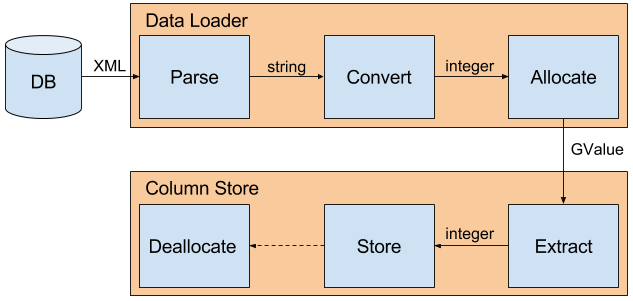
\includegraphics[width=\textwidth]{img/gap-load-original.png}
        \caption{Original implementation where all data is transferred as \cn{GValue}s.}
    \end{subfigure}
    \begin{subfigure}{\textwidth}
        \centering
        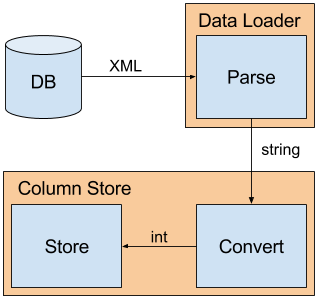
\includegraphics[width=0.52\textwidth]{img/gap-load-raw.png}
        \caption{Enhanced implementation where data is passed to the column store as strings.}
    \end{subfigure}
\caption{By letting the column store accept raw string values from XML, the load process is simplified, and uneccessary memory allocations for \cn{GValues} are removed.}
\label{fig:gap-load-raw}
\end{figure}

In \gap, composition objects in a data source are filled with data using a loading mechanism found in the core event handler. This loader queries the database server and accepts XML values. The loader parses the XML and creates \cn{GValue}s which in turn is sent to the composition objects. Our observation is, with the primitive data type column implementation, that creating \cn{GValue}s when loading a data mart is no longer needed, and those simple type conversions from strings would suffice. This is illustrated in Figure \ref{fig:gap-load-raw}.

\begin{delphicode}{\fn{SetXMLValue} in \cn{PrimitiveFieldValueCollectionBase}.}{lst:primitive-set-xml-value}
procedure PrimitiveFieldValueCollectionBase<TType>.SetXMLValue
( index : integer; xmlValue : string);
begin
  EnsureCapacity(index);
  values[index] := valueHelper.GetFromXMLValue(xmlValue);
  nilFlags[index] := FALSE;
  assignedFlags[index] := TRUE;
end;
\end{delphicode}

To do this, \cn{FieldValueCollectionBase} is extended with a method \cn{LoadXMLValue} that accepts an index and a string xml value. The value helper class is also extended correspondingly, with high performance value conversion functions from the standard library, like \fn{StrToInt} and \fn{StrToFloat}. For more advanced data types, like date, the correct parser functions are called. The implementation is seen in Listing \ref{lst:primitive-set-xml-value}.

We hypothesize that loading XML values directly into a column will speed up load time. We believe this is the case because there will be no allocation and deallocation of \cn{GValues}. Also, as seen in Figure \ref{fig:gap-load-raw}, the new implementation has fewer steps than the original.

\section{Results}
\label{sec:storage-format-test-results}
Like the previous iteration, we test our modifications by using Benchmark \ref{bm:q1}, the \textit{TPC-H Q1 Data Load Benchmark}. We use this benchmark to check our hypothesis that primitive value storage and direct value load contribute to reduced memory footprint and improved load time. 

\cn{GetValue} and \cn{SetValue} in \cn{PrimitiveFieldValueCollection} still use \cn{GValue}, which means memory these values are allocated on access and deallocated when set. We test the effects of this extra memory handling operations with the \textit{Write Benchmark}, benchmark \ref{bm:write}. In addition, the read-intense operations in Benchmark \ref{bm:q1} will also provide insight here.

Full benchmark details are found in Appendix \ref{app:bm}.

%Like last chapter, we test our implementation with Benchmark \ref{bm:q1} and Benchmark \ref{bm:write}. We are curious to see whether memory has been reduced by avoiding the overhead corresponding with \cn{GValue}s and whether load time has been affected. Write performance is also important to test, since \cn{GValue}s are allocated and deallocated as they are read and written to the columns. Full descriptions of the benchmarks are found in Appendix \ref{app:bm}.

\subsection{TPC-H Q1 Data Load Benchmark}
\label{sub:storage-format-tpch-results}
Benchmark \ref{bm:q1}, the \textit{TPC-h Q1 Data Load Benchmark}, was run with our new primitive value column implementation with and without the new loading scheme. Both scaling factor 0.1 and 0.01 were run. Like in Chapter \ref{chap:column-store}, only three tests were run per configuration. However, all results yielded low variance, and no single measurement was more than 15 \% different than the average value.

\begin{table}
    \centering
    \begin{tabularx}{\textwidth}{X | X X}
        & SF0.01 & SF0.1 \\ 
        \hline
        \hline
        Column Store & 419 bytes & 501 bytes \\
        Primitive Column Store & 333 bytes & 374 bytes \\
        Primitive Column Store /w raw load & 381 bytes & 422 bytes \\
    \end{tabularx}
    \caption{Bytes per \texttt{LINEITEM} used by the new primitive value implementation.} 
    \label{tab:primitive-bpl}
\end{table}
As seen in Table \ref{tab:primitive-bpl}, memory is reduced from 419 to 333 bytes and from 501 to 374 bytes for scaling factors 0.01 and 0.1 respectively. This corresponds to 21 \% and 25 \% reduced memory footprint. However, our new loading mechanism increases memory consumption.

\begin{table}
    \centering
    \begin{tabularx}{0.75\textwidth}{X | X X}
        & SF0.01 & SF0.1 \\ 
        \hline
        \hline
        Column Store & 842 ms & 8539 ms \\
        Primitive Column Store & 1210 ms & 13585 ms \\
        Primitive Column Store w/ raw load &  20966 ms & 2306 ms \\
    \end{tabularx}
    \caption{Load times for Benchmark \ref{bm:q1} for the primitive column store for scaling factors 0.01 and 0.1.} 
    \label{tab:primitive-load}
\end{table}
Load times were increased by the primitive column store, but it is still lower than the original implementation. However, with our new loading mechanisms, the load time has increased even more, and is very close to the original implementation. The results are shown in table \ref{tab:non-blackbox-load}. We are surprised to see that our new loading mechanism has degraded load performance. We discuss this in greater detail in Section \ref{sec:part2-discussion}. 

\begin{table}
    \centering
    \begin{tabularx}{\textwidth}{X | X X X | X X X X}
        & \multicolumn{3}{c}{Lookup Index} & \multicolumn{4}{c}{Source Measure Lookup} \\
        \hline
        \hline
        Column Store & 3123 ms & 3301 ms & 13004 ms & 532 ms & 625 ms & 646 ms & 752 ms \\
        Primitive Column Store & 11393 ms & 11960 ms & 19365 ms & 6556 ms & 6856 ms & 6840 ms & 6826 ms \\
    \end{tabularx}
    \caption{Data mart load operation times for \ref{bm:q1} with the primitive columns.} 
    \label{tab:primitive-q1}
\end{table}
Most operations are drastically slowed down by the new primitive storage format, as seen in Table \ref{tab:primitive-q1}. Source measure lookup is ten times slower than the previous column store implementation, and almost 20 times slower as the original implementation.

\subsection{Write Benchmark}
\label{sub:Write Benchmark}
\begin{table}
    \begin{tabularx}{\textwidth}{X | X X X X}
         & \texttt{QUANTITY} & \texttt{EXTENDEDPRICE} & \texttt{COMMENT} & \texttt{SHIPDATE}\\ 
        \hline
        \hline
        Column Store & 1642 ms & 1610 ms & 1770 ms & 2046 ms \\
        Primitive Column Store & 1807 ms & 1779 ms & 1820 ms & 2352 ms \\
    \end{tabularx}
    \caption{Test results for Benchmark \ref{bm:write}.}
    \label{tab:primitive-write}
\end{table}
Write performance has, as Table \ref{tab:primitive-write} shows, degraded slightly with the new primitive data type column store. No operations are more than 15 \% slower than the original.

\section{Discussion}
\label{sec:part2-discussion}

We see that memory used per \lineitem~for SF0.1 has been reduced by an additional 25 \% compared to the \cn{FieldValueCollection} implementation. This observation means the overhead associated with \cn{GValue}s is significant.

We observe an increased load time for Benchmark \ref{bm:q1}, where the time it takes to populate the data source is increased from 8.5 seconds to 13.6 seconds. We believe the extra steps needed to extract raw values from \cn{GValue} instances causes this. Still, the load time is lower than the original \gap~implementation.

Circumventing \cn{GValue} creation and loading raw XML string values directly into the column store had no positive effect on the \textit{TPC-H Q1 Data Load Benchmark}. Here, both the number of bytes per \lineitem~and load time increased. We did circumvent the creation of \cn{GValue}s, but by doing so, we also disabled the existing caching mechanism in \gap. Thus, no strings are reused, and no conversion results are cached. It is likely that this is the cause of increased memory usage and load time.

We see the consequences of having a \cn{GValue} interface with the columns, which results in frequent allocations and deallocations when accessing values. The \textit{write benchmark} shows slightly reduced write performance. However, we measure the largest performance impact on the read-intensive operations in the \textit{TPC-H Q1 Data Load Benchmark}. For source measure lookup, which creates a real value array for a column using a tight loop, the performance has dropped and is now ten times slower than the \cn{FieldValueCollection} column store due to the frequent memory allocations.

%The extra steps of \cn{GValue} allocation and deallocation also affects write performance in Benchmark \ref{bm:write}, although not by more than 15 \%. This indicates that there are much more overhead associated with data write than just allocating \cn{GValue}s.

\section{Iteration Conclusion}
\label{sec:Iteration Conclusion}
We conclude that primitive value column storage successfully reduces memory consumption in \gap. Compared to the original implementation, the bytes used per \lineitem~are reduced from 715 bytes to 374 bytes. Our changes have affected write performance negatively, but not by more than 15 \%. We argue that the significant reduction in memory usage outweighs the slightly negative impact on write performance, and concludes that storing values as primitive data types and using a \cn{GValue} interface is feasible. 

In this iteration, we have laid an important foundation for optimizing the read-intensive operations in the \textit{TPC-H Q1 Data Load Benchmark} by increasing data locality. More specifically, we have replaced the \cn{GValue} pointers and now store values directly in the columns. Until we exploit this storage structure, source measure lookup and lookup index generation, suffer severely due to memory allocation operations on each access. We investigate column operations in Chapter \ref{chap:operations}.

Our hypothesis that loading data as raw XML values into the column would reduce load time was wrong, at least for now. Circumventing \cn{GValue}s also circumvents the built-in caching mechanism in \gap~and results in higher memory usage and slower load times.  

We have cut the application memory requirements in half without applying any form of compression. Now that we know data can be stored as primitive data types, the next step is to compress the data with techniques used by read-optimized databases.

\subsection{Future Work}
\label{sub:Future Work}
We are still keen to investigate the potential of loading XML values directly, but due to time constraints, we are unable to pursue this topic further. Future work should aim to replicate the existing caching mechanisms in \gap, but within the column store and without creation of \cn{GValue}s. Caching could, for instance, only be enabled if the data source is in a feeding state.
